\documentclass[11pt,a4paper]{article}
\usepackage[utf8]{inputenc}
\usepackage[margin=1in]{geometry}
\usepackage{amsmath}
\usepackage{amssymb}
\usepackage{graphicx}
\usepackage{hyperref}
\usepackage{listings}
\usepackage{xcolor}
\usepackage{booktabs}
\usepackage{float}

% Python code styling
\lstset{
    language=Python,
    basicstyle=\ttfamily\small,
    keywordstyle=\color{blue},
    commentstyle=\color{gray},
    stringstyle=\color{red},
    showstringspaces=false,
    breaklines=true,
    frame=single,
    backgroundcolor=\color{gray!10}
}

\title{Machine Learning Assignment 2\\Lasso and Ridge Regression}
\author{Dataset ID: 23-23--23}
\date{}

\begin{document}

\maketitle

In this assignment I've used Lasso and Ridge regression on a dataset with polynomial features to understand how regularization works and how to pick the best hyperparameter using cross-validation. The dataset has 199 data points with two input features ($x_1$, $x_2$) and one target variable ($y$).

\section*{Part (i): Training Lasso and Ridge Models}

\subsection*{(i)(a) Looking at the Data}

First I loaded the data and plotted it in 3D to see what it looks like:

\begin{lstlisting}
import numpy as np
import matplotlib.pyplot as plt
from mpl_toolkits.mplot3d import Axes3D

data = np.loadtxt('week3.csv', delimiter=',', skiprows=1)
X = data[:, :2]
y = data[:, 2]

fig = plt.figure()
ax = fig.add_subplot(111, projection='3d')

# plot points colored by target value
scatter = ax.scatter(X[:,0], X[:,1], y, c=y, cmap='viridis', s=30)

ax.set_xlabel('Feature 1 (x1)')
ax.set_ylabel('Feature 2 (x2)')
ax.set_zlabel('Target (y)')
ax.set_title('3D Scatter Plot')

# add colorbar
plt.colorbar(scatter, ax=ax, shrink=0.5, aspect=5, label='Target (y)')

plt.show()
\end{lstlisting}

The points are colored by their target value using the viridis colormap - darker colors represent lower $y$ values and brighter colors represent higher $y$ values. This color coding helps visualize how the target changes across the feature space.

\textbf{Does the data lie on a plane or curve?}

Looking at the scatter plot, the data definitely looks curved, not flat. You can see from the color gradient that the target values follow a non-linear pattern across the feature space. If I tried fitting just a plane (linear model) to this it wouldn't work well. This tells me I need polynomial features to capture the non-linear patterns.

\begin{figure}[H]
\centering
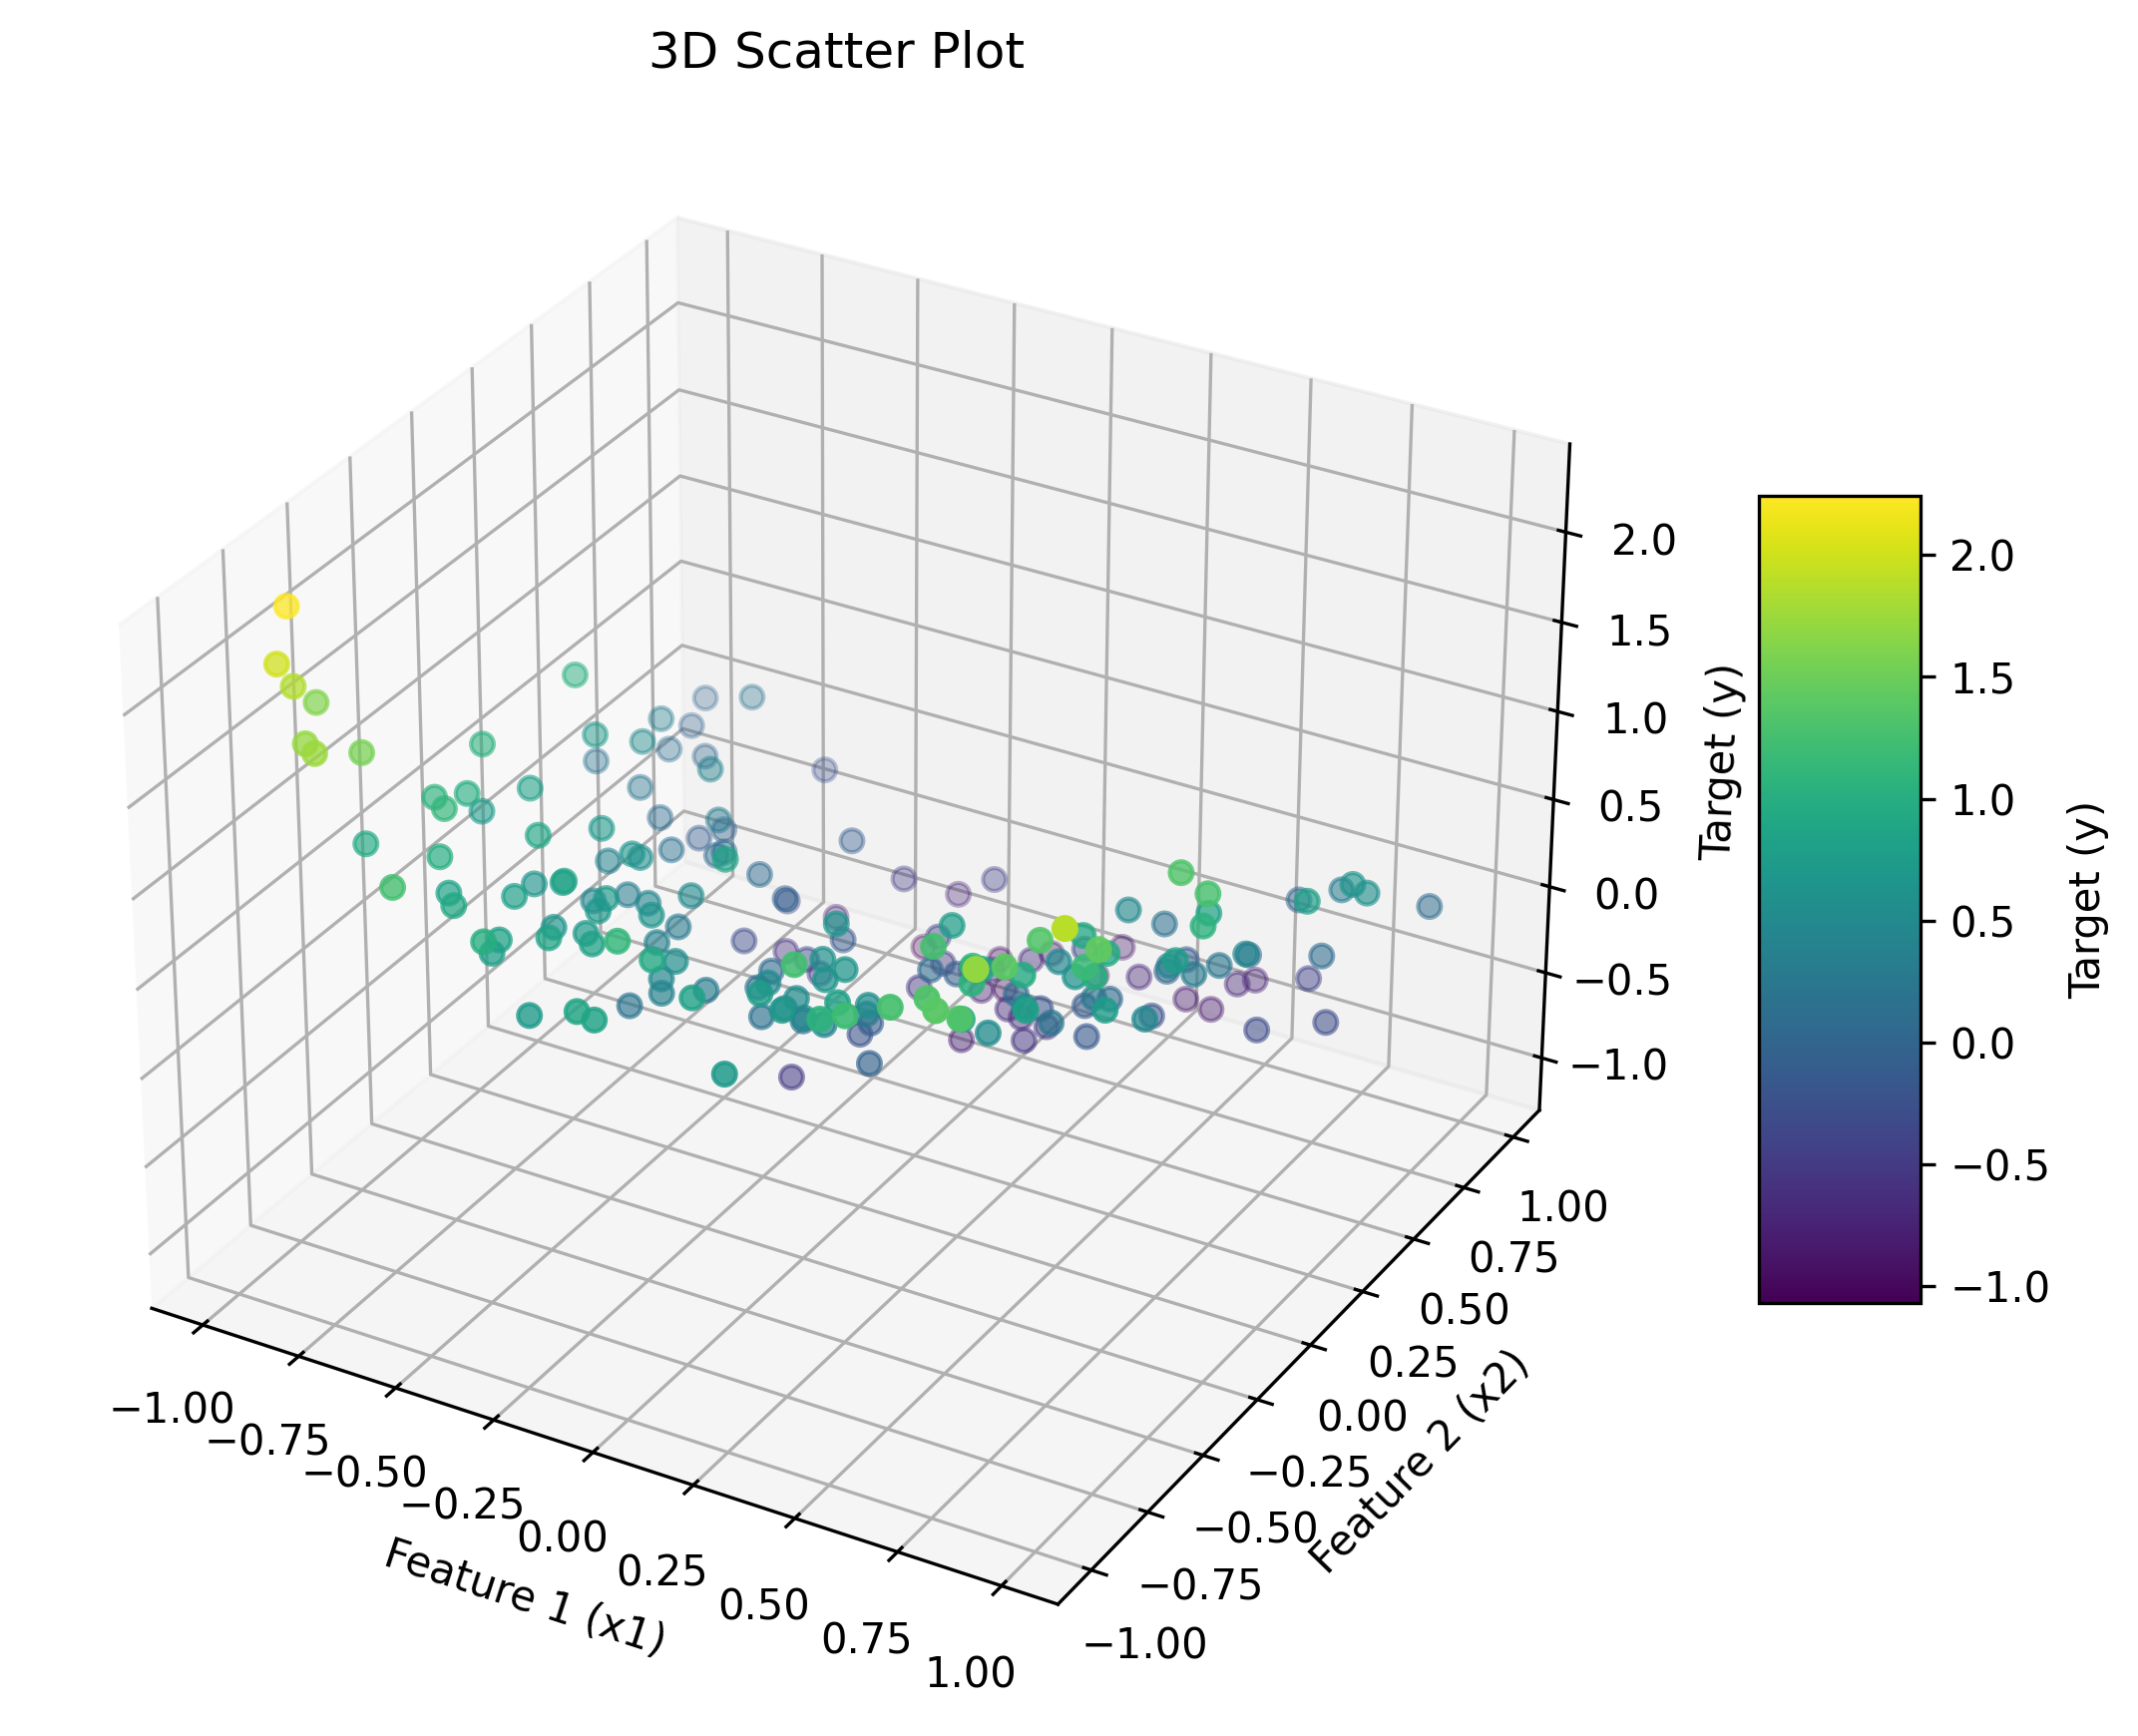
\includegraphics[width=0.7\textwidth]{figures/02_3d_scatter_plot.png}
\caption{3D scatter plot of the data with points colored by target value using the viridis colormap.}
\label{fig:3d_scatter}
\end{figure}

\subsection*{(i)(b) Lasso with Polynomial Features}

I created polynomial features up to degree 5, which gives 21 features total:

\begin{lstlisting}
from sklearn.preprocessing import PolynomialFeatures
from sklearn.linear_model import Lasso

poly = PolynomialFeatures(degree=5, include_bias=True)
Xpoly = poly.fit_transform(X)
\end{lstlisting}

The 21 features are: 1, $x_1$, $x_2$, $x_1^2$, $x_1x_2$, $x_2^2$, $x_1^3$, $x_1^2x_2$, $x_1x_2^2$, $x_2^3$, $x_1^4$, $x_1^3x_2$, $x_1^2x_2^2$, $x_1x_2^3$, $x_2^4$, $x_1^5$, $x_1^4x_2$, $x_1^3x_2^2$, $x_1^2x_2^3$, $x_1x_2^4$, $x_2^5$

Then I trained Lasso models with different $C$ values. Remember that sklearn uses $\alpha = 1/(2C)$, so:

\begin{lstlisting}
C_values = [0.001, 0.01, 0.1, 1, 10, 100, 1000]

for C in C_values:
    model = Lasso(alpha=1/(2*C), max_iter=10000)
    model.fit(Xpoly, y)
\end{lstlisting}

\textbf{Results:}

\begin{table}[H]
\centering
\begin{tabular}{ccc}
\toprule
C & Non-zero Coefficients & Training MSE \\
\midrule
0.001 & 0 & 0.4574 \\
0.01 & 0 & 0.4574 \\
0.1 & 0 & 0.4574 \\
1 & 0 & 0.4574 \\
10 & 2 & 0.0772 \\
100 & 2 & 0.0392 \\
1000 & 10 & 0.0368 \\
\bottomrule
\end{tabular}
\end{table}

\textbf{What's happening as C changes?}

When $C$ is small (0.001 to 1), the regularization is really strong - so strong that ALL coefficients get pushed to zero. The model just predicts a constant value, which gives bad MSE.

At $C=10$, finally two coefficients become non-zero: $x_2$ and $x_1^2$. As $C$ increases further (100, 1000), more coefficients become non-zero and the training error goes down.

\textbf{Detailed coefficients for all C values:}

\begin{table}[H]
\centering
\small
\begin{tabular}{lccccccc}
\toprule
Feature & C=0.001 & C=0.01 & C=0.1 & C=1 & C=10 & C=100 & C=1000 \\
\midrule
$x_2$ & 0 & 0 & 0 & 0 & -0.845 & -0.988 & -1.049 \\
$x_1^2$ & 0 & 0 & 0 & 0 & 0.510 & 1.060 & 1.109 \\
$x_1x_2$ & 0 & 0 & 0 & 0 & 0 & 0 & -0.180 \\
$x_1^3$ & 0 & 0 & 0 & 0 & 0 & 0 & -0.012 \\
$x_1^2x_2$ & 0 & 0 & 0 & 0 & 0 & 0 & 0.045 \\
$x_1^3x_2$ & 0 & 0 & 0 & 0 & 0 & 0 & 0.213 \\
$x_1^4x_2$ & 0 & 0 & 0 & 0 & 0 & 0 & -0.094 \\
$x_1^3x_2^2$ & 0 & 0 & 0 & 0 & 0 & 0 & -0.008 \\
$x_1x_2^4$ & 0 & 0 & 0 & 0 & 0 & 0 & -0.033 \\
$x_2^5$ & 0 & 0 & 0 & 0 & 0 & 0 & 0.125 \\
\bottomrule
\end{tabular}
\end{table}

This is the $L_1$ penalty in action - it forces coefficients to be exactly zero, not just small. This is called \textit{feature selection}.

\subsection*{(i)(c) Visualizing Predictions}

I generated predictions on a grid that extends beyond the training data range (as required). My data goes from about -1 to 1, so I extended the grid to about -3 to 3:

\begin{lstlisting}
x1_range = X[:,0].max() - X[:,0].min()
x2_range = X[:,1].max() - X[:,1].min()
x1_min = X[:,0].min() - 1.0*x1_range
x1_max = X[:,0].max() + 1.0*x1_range
x2_min = X[:,1].min() - 1.0*x2_range
x2_max = X[:,1].max() + 1.0*x2_range

x1_grid = np.linspace(x1_min, x1_max, 60)
x2_grid = np.linspace(x2_min, x2_max, 60)
X1_mesh, X2_mesh = np.meshgrid(x1_grid, x2_grid)

Xg = np.c_[X1_mesh.ravel(), X2_mesh.ravel()]
Xg_poly = poly.transform(Xg)
Z = model.predict(Xg_poly).reshape(X1_mesh.shape)

fig = plt.figure()
ax = fig.add_subplot(111, projection='3d')
ax.plot_surface(X1_mesh, X2_mesh, Z, alpha=0.6, cmap='viridis')
ax.scatter(X[:,0], X[:,1], y, c='red', s=30)
plt.show()
\end{lstlisting}

I plotted surfaces for $C = 0.001$, $C = 1$, and $C = 1000$.

\textbf{What I see:}

\begin{itemize}
    \item \textbf{C = 0.001}: Almost completely flat surface. The model is totally underfitting - it's just predicting roughly the mean value everywhere because all coefficients are zero.
    
    \item \textbf{C = 1}: Still flat. Same problem - regularization is too strong.
    
    \item \textbf{C = 1000}: Now we see a curved surface that fits the data points pretty well. The model is complex enough to capture the patterns. Maybe a bit too complex though - could be starting to overfit.
\end{itemize}

The plots clearly show that as $C$ increases, the prediction surface goes from flat (underfitting) to curved (better fit).

\begin{figure}[H]
\centering
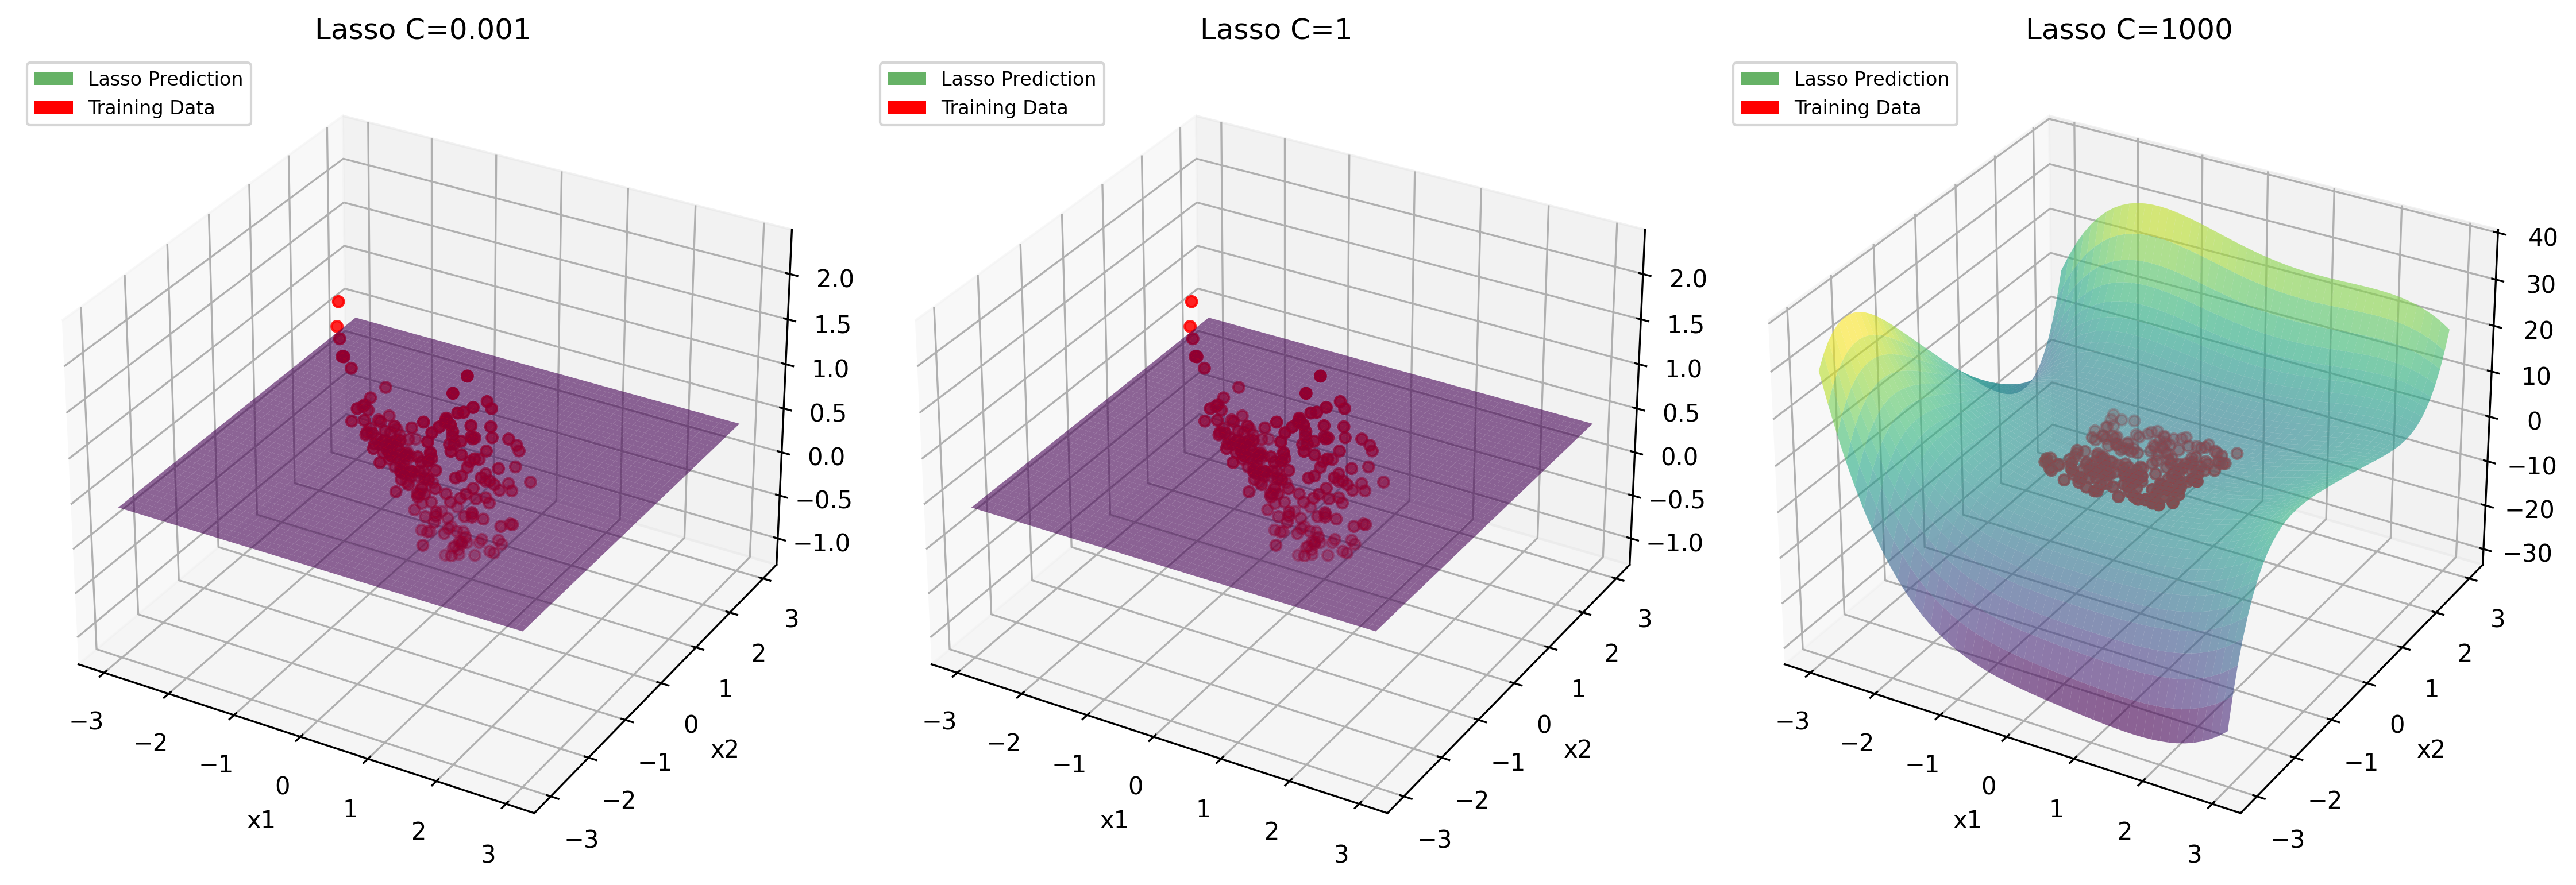
\includegraphics[width=0.95\textwidth]{figures/03_lasso_prediction_surfaces.png}
\caption{Lasso prediction surfaces for different C values (0.001, 1, 1000). The surfaces (colored) show model predictions on an extended grid, and red points show the training data.}
\label{fig:lasso_surfaces}
\end{figure}

\subsection*{(i)(d) Underfitting vs Overfitting}

\textbf{What is underfitting?} When your model is too simple to capture the actual patterns in the data. In Lasso, this happens when $C$ is too small and regularization is too strong. You get high bias (model is biased toward being too simple) and low variance (predictions don't change much with different training sets). Both training error and test error are high.

\textbf{What is overfitting?} When your model is too complex and starts fitting the noise in the training data instead of just the real pattern. Happens when $C$ is too large. You get low bias but high variance (predictions change a lot with different training sets). Training error is low but test error is high.

\textbf{How C controls this trade-off:}

The $C$ parameter controls the strength of regularization through the penalty term:

\begin{equation}
J(\theta) = \frac{1}{m} \sum_{i=1}^{m} (h_\theta(x^{(i)}) - y^{(i)})^2 + \frac{1}{C} \sum_{j=1}^{n} |\theta_j|
\end{equation}

\begin{itemize}
    \item \textbf{Small C} $\rightarrow$ large penalty $\rightarrow$ strong regularization $\rightarrow$ fewer non-zero coefficients $\rightarrow$ simpler model $\rightarrow$ underfitting
    \item \textbf{Large C} $\rightarrow$ small penalty $\rightarrow$ weak regularization $\rightarrow$ more non-zero coefficients $\rightarrow$ complex model $\rightarrow$ overfitting
\end{itemize}

From my results:
\begin{itemize}
    \item $C \leq 1$: Definitely underfitting (0 non-zero coefficients, MSE = 0.4574)
    \item $C = 10$: Starting to fit (2 coefficients, MSE = 0.0772)
    \item $C = 100$: Good fit (2 coefficients, MSE = 0.0392)
    \item $C = 1000$: Possibly overfitting (10 coefficients, MSE = 0.0368)
\end{itemize}

The sweet spot is somewhere around $C = 10$-$100$ where we balance complexity and regularization.

\begin{figure}[H]
\centering
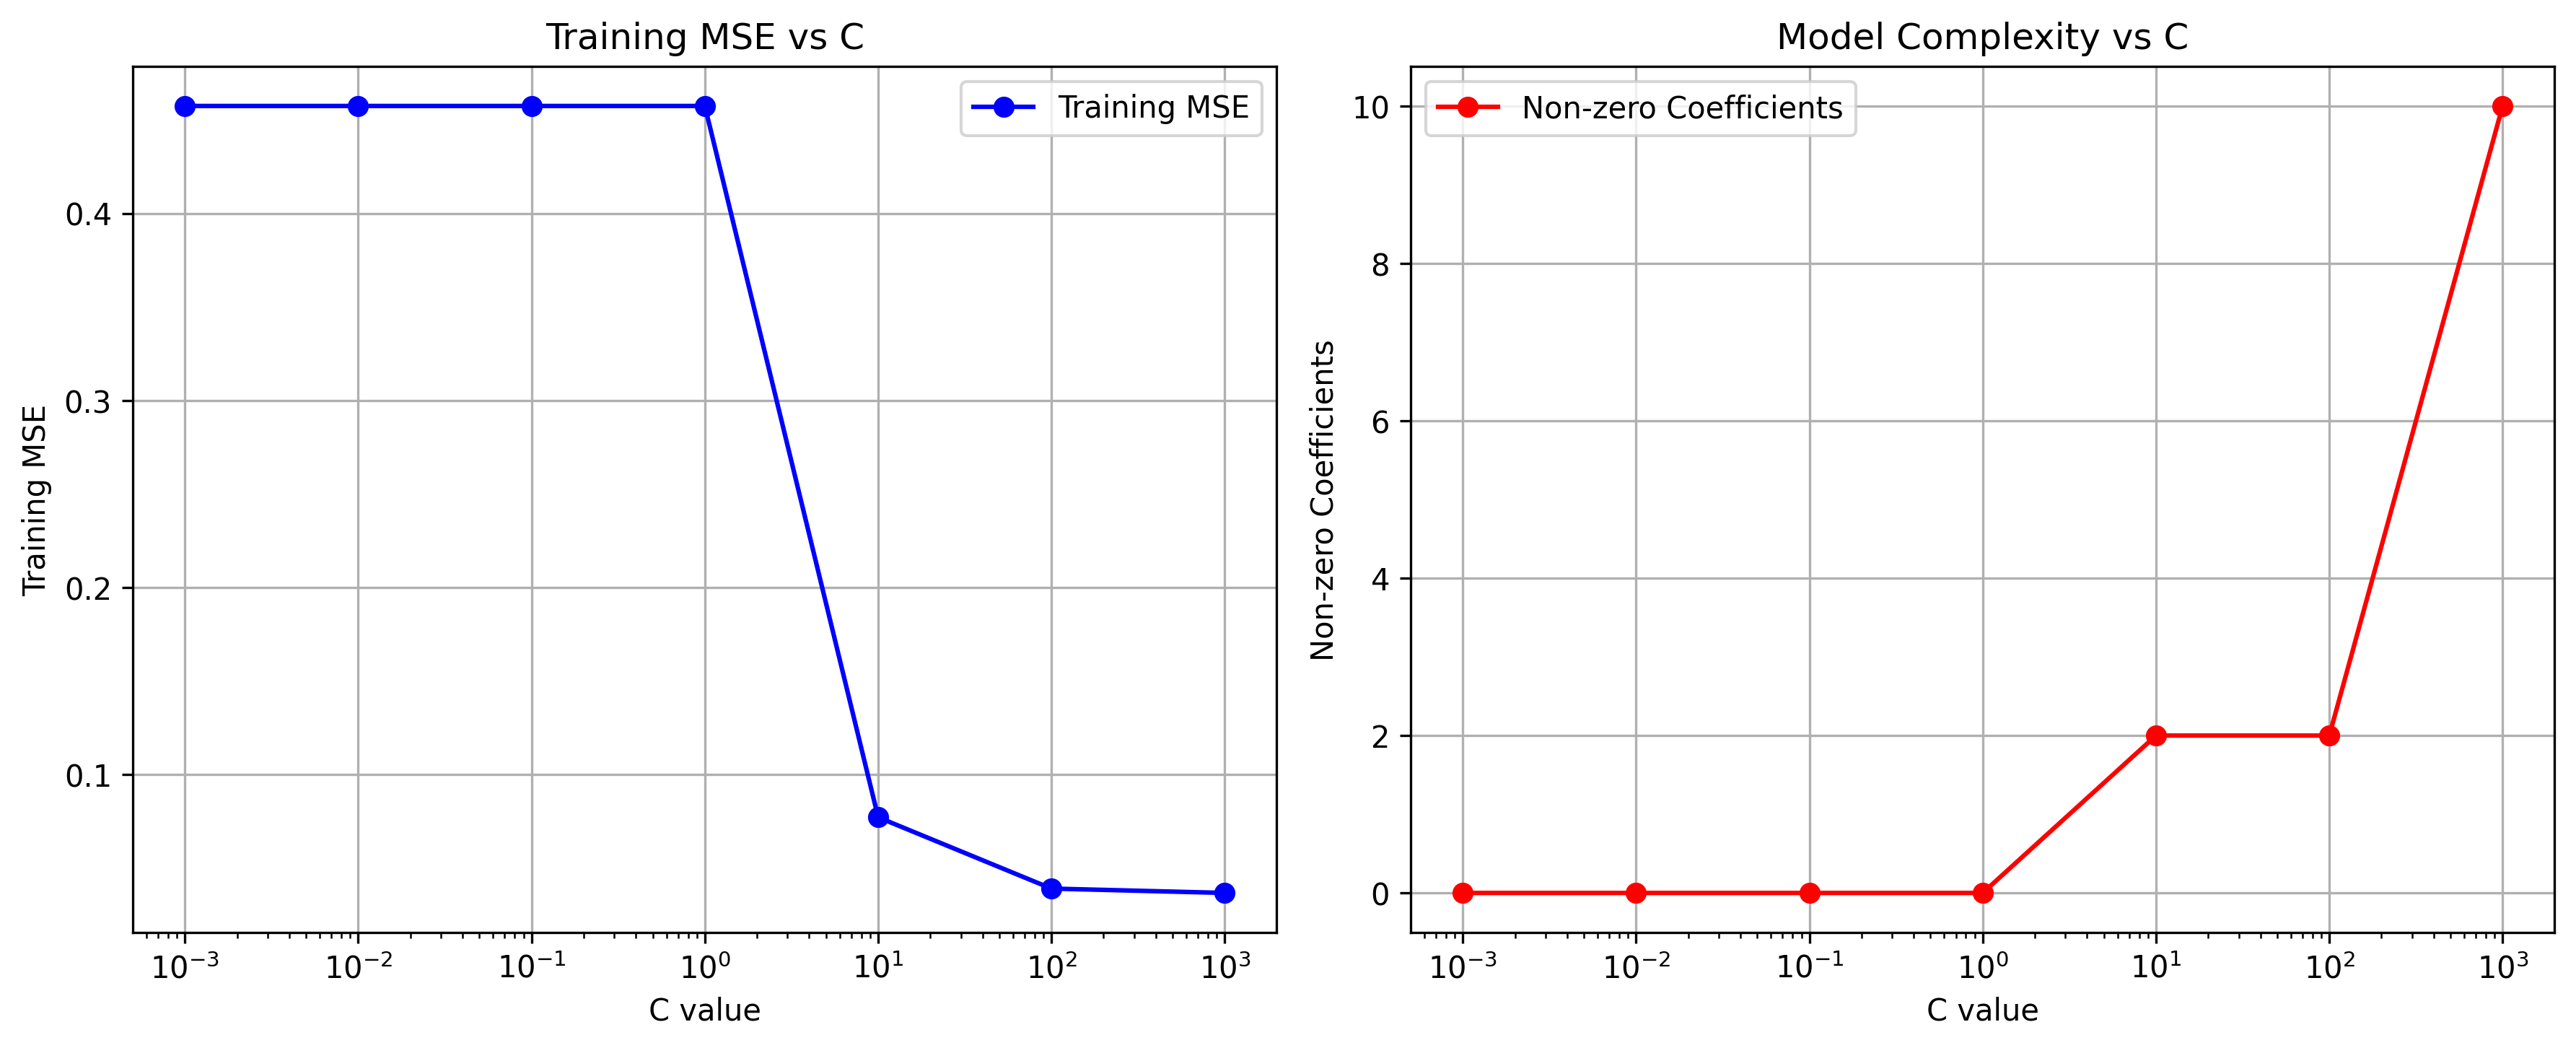
\includegraphics[width=0.95\textwidth]{figures/04_underfitting_overfitting_analysis.png}
\caption{Left: Training MSE decreases as C increases (less regularization). Right: Number of non-zero coefficients increases with C, showing the model becoming more complex.}
\label{fig:underfitting_overfitting}
\end{figure}

\subsection*{(i)(e) Ridge Regression Comparison}

Ridge regression uses $L_2$ penalty instead of $L_1$:

\begin{equation}
J(\theta) = \frac{1}{m} \sum_{i=1}^{m} (h_\theta(x^{(i)}) - y^{(i)})^2 + \frac{1}{C} \theta^T\theta
\end{equation}

\begin{lstlisting}
from sklearn.linear_model import Ridge

for C in C_values:
    model = Ridge(alpha=1/(2*C))
    model.fit(Xpoly, y)
\end{lstlisting}

\textbf{Ridge Results:}

\begin{table}[H]
\centering
\begin{tabular}{cc}
\toprule
C & Training MSE \\
\midrule
0.001 & 0.3467 \\
0.01 & 0.1211 \\
0.1 & 0.0455 \\
1 & 0.0370 \\
10 & 0.0351 \\
100 & 0.0349 \\
1000 & 0.0349 \\
\bottomrule
\end{tabular}
\end{table}

\textbf{Key Differences Between Lasso and Ridge:}

\begin{enumerate}
    \item \textbf{Sparsity}: This is the big one. Lasso sets coefficients to \textit{exactly} zero ($L_1$ penalty), while Ridge just makes them small ($L_2$ penalty). You can see this at $C=1$:
\end{enumerate}

\begin{table}[H]
\centering
\small
\begin{tabular}{lcc|lcc}
\toprule
Feature & Lasso & Ridge & Feature & Lasso & Ridge \\
\midrule
1 & 0.000 & -0.809 & $x_1^3x_2$ & 0.000 & 0.183 \\
$x_1$ & 0.000 & -0.003 & $x_1^2x_2^2$ & 0.000 & 0.034 \\
$x_2$ & 0.000 & -1.019 & $x_1x_2^3$ & 0.000 & 0.055 \\
$x_1^2$ & 0.000 & 0.909 & $x_2^4$ & 0.000 & 0.034 \\
$x_1x_2$ & 0.000 & -0.199 & $x_1^5$ & 0.000 & 0.087 \\
$x_2^2$ & 0.000 & -0.051 & $x_1^4x_2$ & 0.000 & -0.149 \\
$x_1^3$ & 0.000 & -0.076 & $x_1^3x_2^2$ & 0.000 & -0.103 \\
$x_1^2x_2$ & 0.000 & 0.088 & $x_1^2x_2^3$ & 0.000 & -0.037 \\
$x_1x_2^2$ & 0.000 & 0.118 & $x_1x_2^4$ & 0.000 & -0.112 \\
$x_2^3$ & 0.000 & -0.062 & $x_2^5$ & 0.000 & 0.154 \\
$x_1^4$ & 0.000 & 0.198 & & & \\
\bottomrule
\end{tabular}
\caption*{Coefficient comparison at C=1: Lasso has all zeros (strong regularization), while Ridge has small non-zero values for all 21 features.}
\end{table}

\begin{enumerate}
    \setcounter{enumi}{1}
    \item \textbf{Training Error}: Ridge generally achieves lower training MSE than Lasso for the same $C$ value.
    
    \item \textbf{Interpretability}: Lasso gives you automatic feature selection - easier to interpret because you know which features matter. Ridge keeps everything.
\end{enumerate}

\textbf{When to use which?}

\begin{itemize}
    \item Use \textbf{Lasso} when you think only a few features really matter and you want automatic feature selection
    \item Use \textbf{Ridge} when you think most features contribute something and you just want to shrink them
\end{itemize}

\begin{figure}[H]
\centering
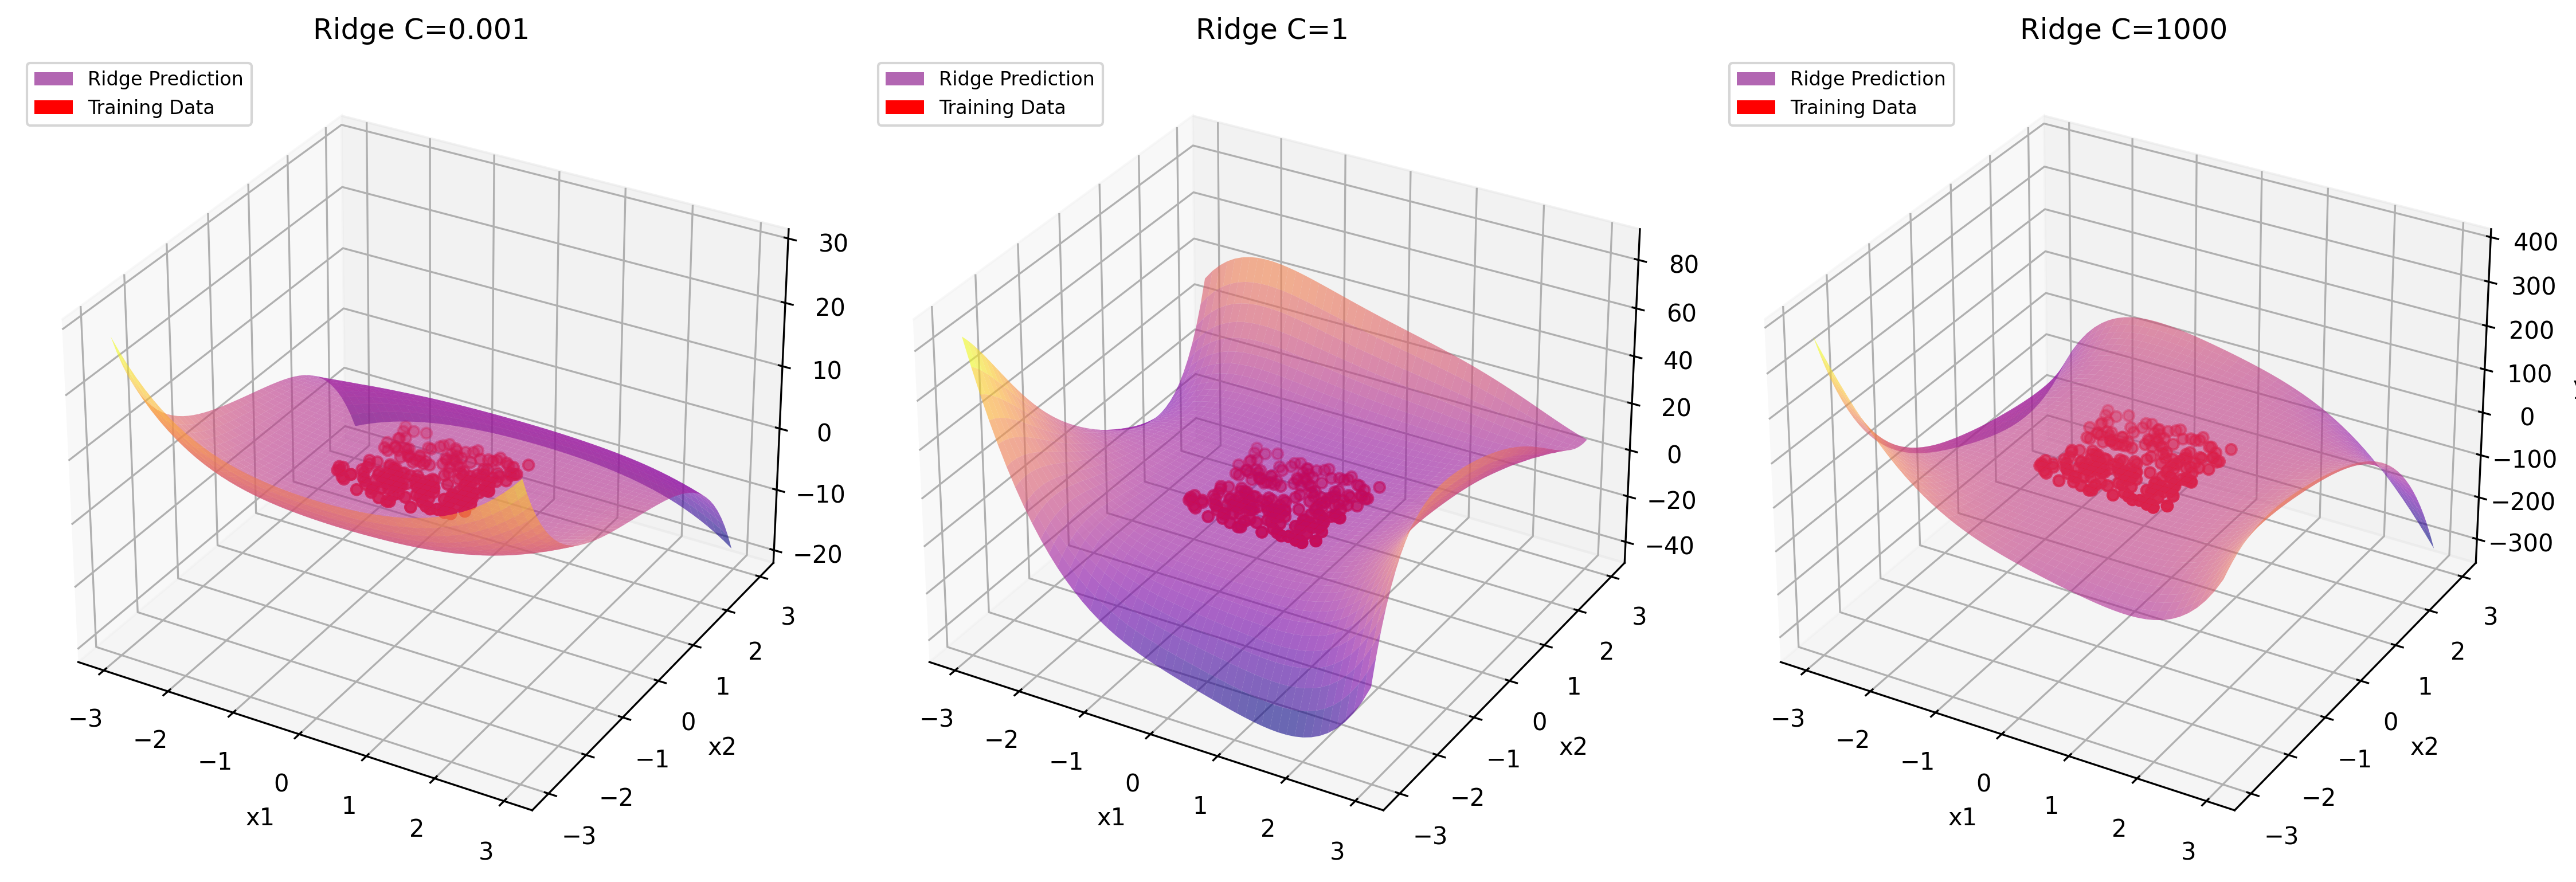
\includegraphics[width=0.95\textwidth]{figures/05_ridge_prediction_surfaces.png}
\caption{Ridge prediction surfaces for different C values (0.001, 1, 1000). Unlike Lasso, Ridge produces smooth transitions between regularization levels without setting coefficients to exactly zero.}
\label{fig:ridge_surfaces}
\end{figure}

\section*{Part (ii): Cross-Validation for Hyperparameter Selection}

\subsection*{(ii)(a) 5-Fold Cross-Validation for Lasso}

I used 5-fold CV to find the best $C$ value. Split the data into 5 parts, train on 4 parts and test on the 5th, repeat for all combinations:

\begin{lstlisting}
from sklearn.model_selection import KFold

kf = KFold(n_splits=5, shuffle=True, random_state=42)
C_cv = [0.001, 0.01, 0.1, 0.5, 1, 2, 5, 10, 50, 100, 500, 1000]

cv_means = []
cv_stds = []

for C in C_cv:
    scores = []
    for train_idx, val_idx in kf.split(Xpoly):
        model = Lasso(alpha=1/(2*C), max_iter=10000)
        model.fit(Xpoly[train_idx], y[train_idx])
        pred = model.predict(Xpoly[val_idx])
        scores.append(mean_squared_error(y[val_idx], pred))
    
    cv_means.append(np.mean(scores))
    cv_stds.append(np.std(scores))

plt.errorbar(C_cv, cv_means, yerr=cv_stds, fmt='o-', capsize=5)
plt.xscale('log')
plt.xlabel('C value')
plt.ylabel('CV MSE')
plt.show()
\end{lstlisting}

\textbf{Why this range of C values?}

I started small (0.001) where regularization is super strong, and went up to 1000 where it's very weak. Used 12 different values to get a good picture of what's happening. The lecture notes suggest increasing by factors of 5 or 10, which is roughly what I did.

\textbf{CV Results:}

\begin{table}[H]
\centering
\begin{tabular}{ccc}
\toprule
C & Mean CV MSE & Std Dev \\
\midrule
0.001 & 0.4670 & 0.1241 \\
0.01 & 0.4670 & 0.1241 \\
0.1 & 0.4670 & 0.1241 \\
0.5 & 0.4670 & 0.1241 \\
1 & 0.4670 & 0.1241 \\
2 & 0.3571 & 0.1239 \\
5 & 0.1801 & 0.0552 \\
10 & 0.0814 & 0.0260 \\
50 & 0.0416 & 0.0119 \\
\textbf{100} & \textbf{0.0408} & \textbf{0.0119} \\
500 & 0.0419 & 0.0135 \\
1000 & 0.0429 & 0.0146 \\
\bottomrule
\end{tabular}
\end{table}

The error bars show the standard deviation across the 5 folds. This tells us how stable the model is - a small standard deviation means the model performs consistently across different train/test splits, while a large standard deviation suggests the model's performance varies a lot depending on which data it sees. This helps us choose not just the model with lowest mean error, but also one that's reliable.

\begin{figure}[H]
\centering
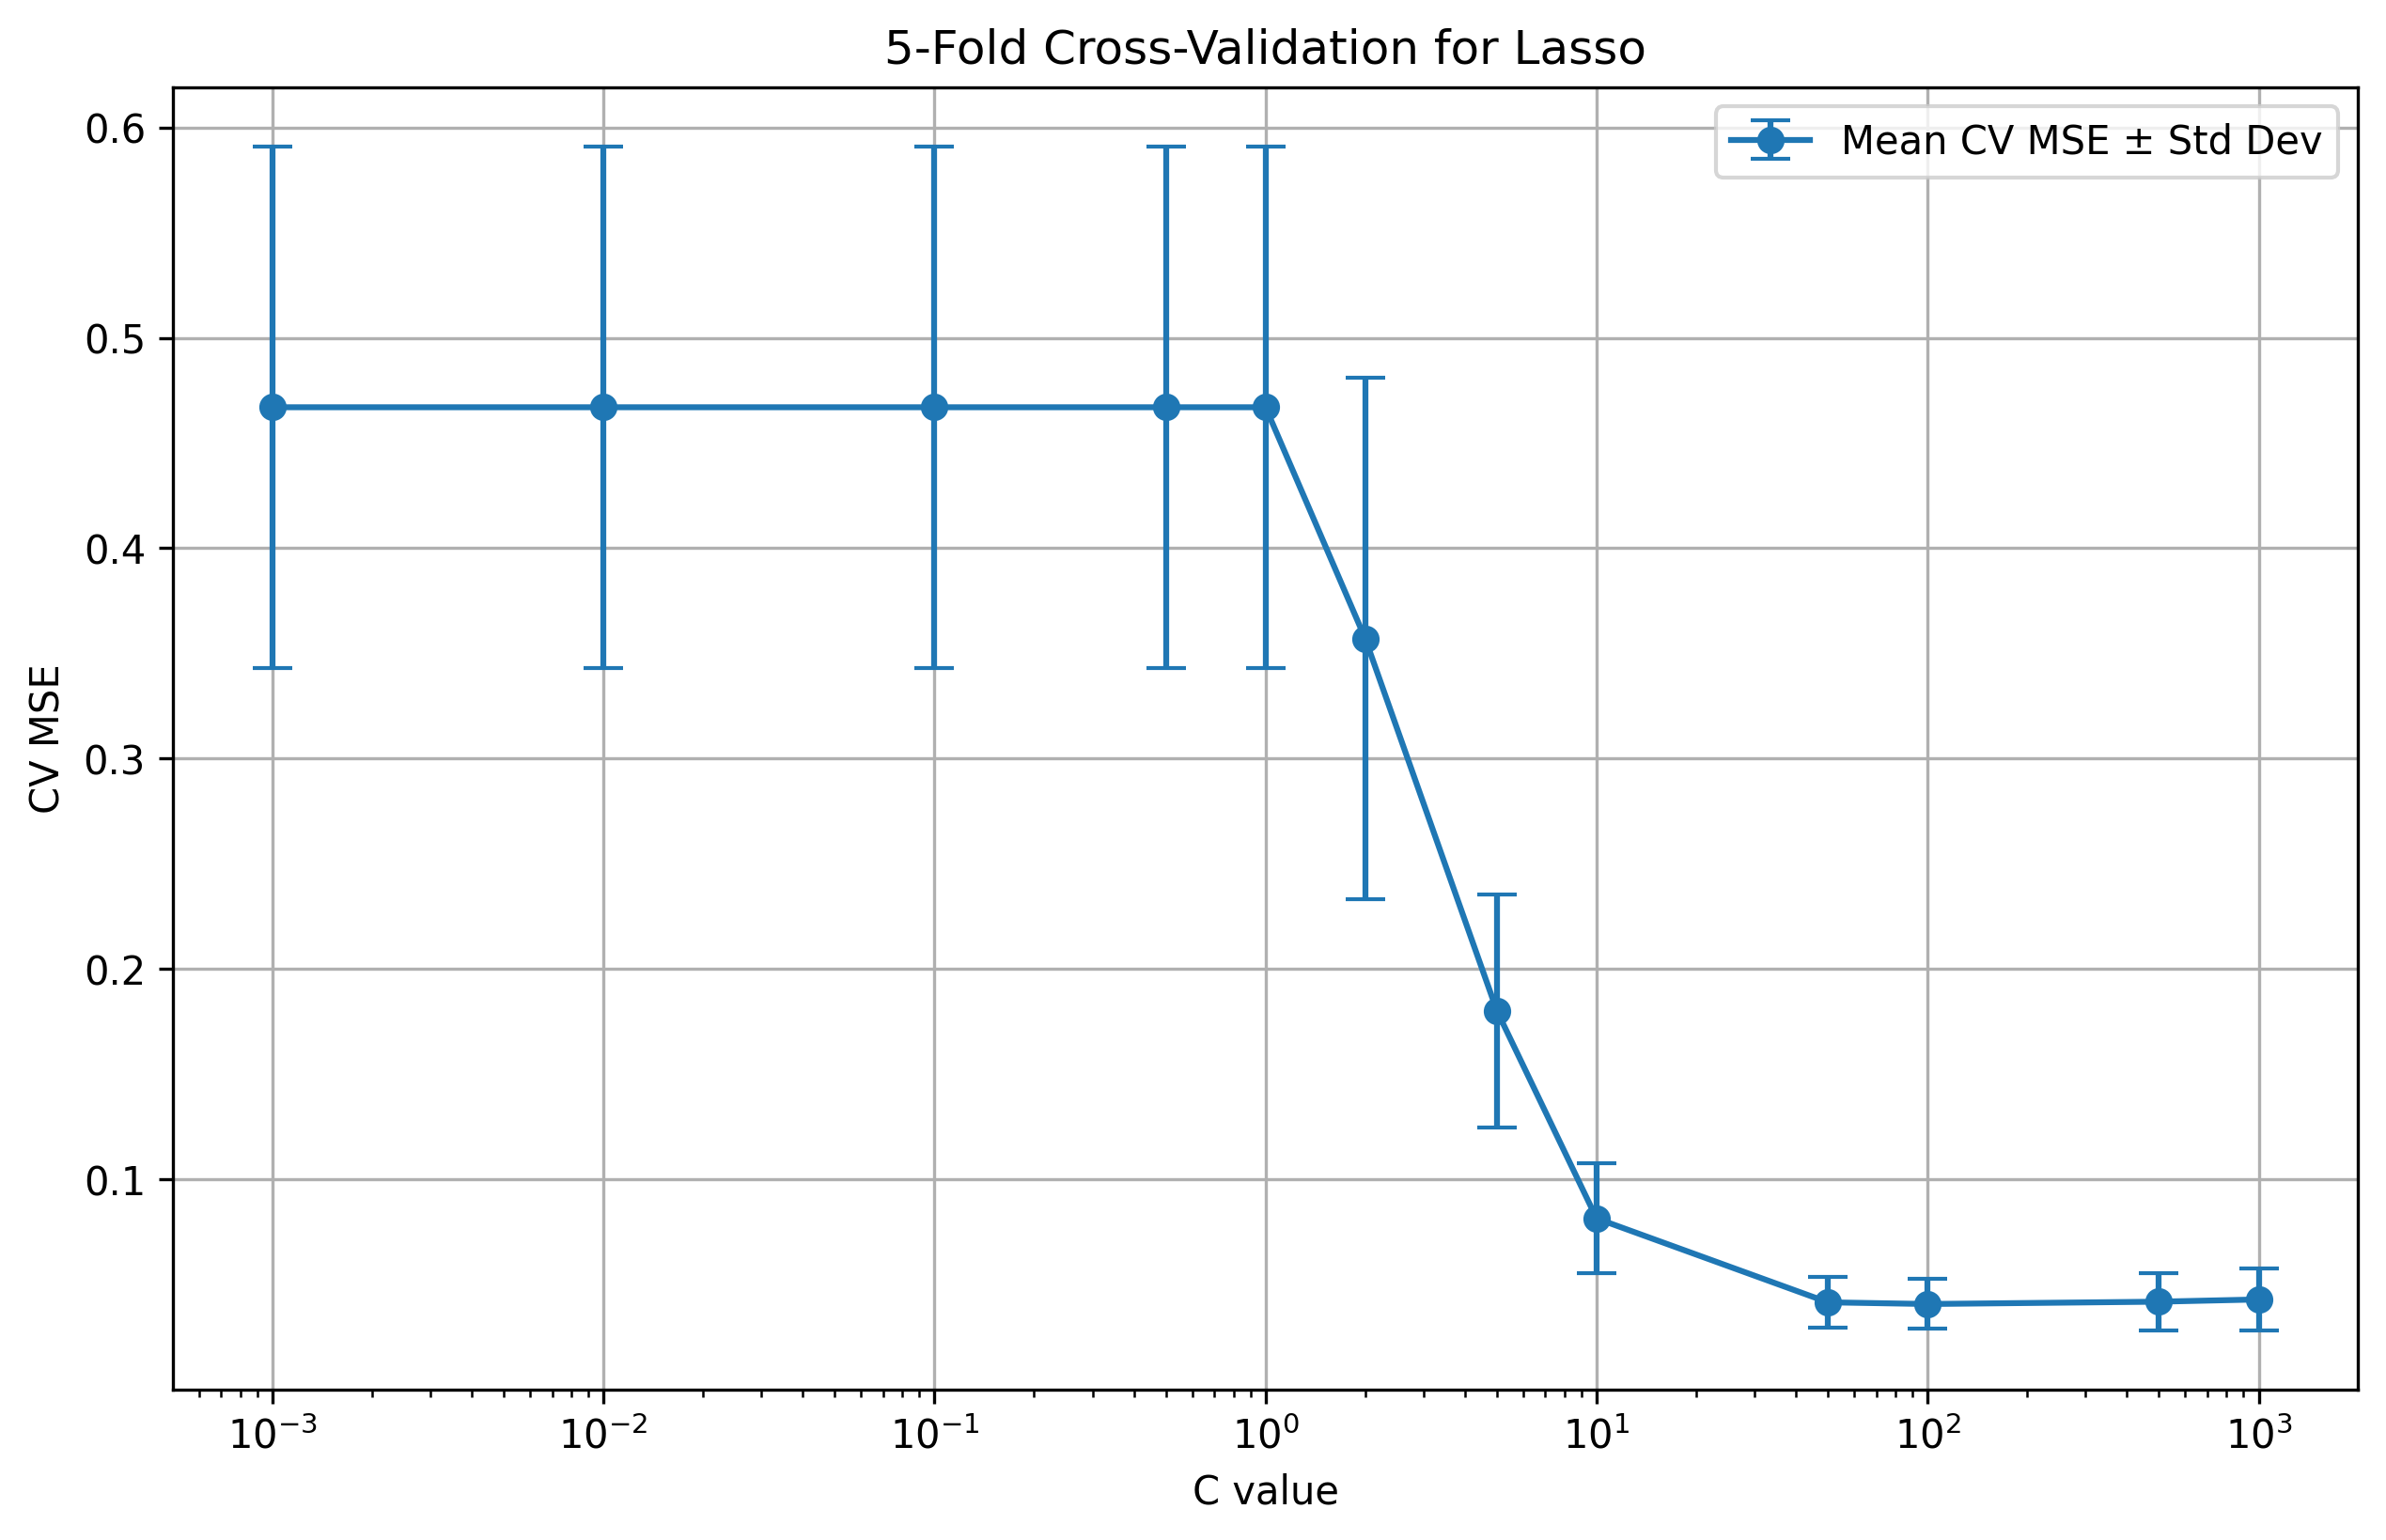
\includegraphics[width=0.8\textwidth]{figures/06_lasso_cv_results.png}
\caption{5-fold cross-validation results for Lasso. The error bars represent standard deviation across folds. The optimal C value is 100, where CV MSE is minimized.}
\label{fig:lasso_cv}
\end{figure}

\subsection*{(ii)(b) Recommended C Value for Lasso}

\textbf{Best C = 100}

\textbf{Why?}
\begin{itemize}
    \item It has the lowest cross-validation MSE: 0.0408
    \item The standard deviation is reasonable (0.0119), so it's stable
    \item Looking at the plot, $C=50$ and $C=100$ are pretty close, but $C=100$ edges it slightly
    \item After $C=100$, the error starts going back up, which suggests we'd be overfitting
\end{itemize}

\textbf{Final Lasso Model (C=100):}
\begin{itemize}
    \item CV MSE: $0.0408 \pm 0.0119$
    \item Non-zero coefficients: 2 out of 21
    \item The two features selected: $x_2$ and $x_1^2$
    \item Coefficients: 
    \begin{itemize}
        \item $x_2$: -0.987955
        \item $x_1^2$: 1.060313
    \end{itemize}
\end{itemize}

This is a really nice sparse solution - out of 21 possible features, Lasso picked just 2 that actually matter. Makes sense given what we saw in the 3D plot.

\subsection*{(ii)(c) Cross-Validation for Ridge}

Did the same thing for Ridge:

\begin{lstlisting}
ridge_cv_means = []
ridge_cv_stds = []

for C in C_cv:
    scores = []
    for train_idx, val_idx in kf.split(Xpoly):
        model = Ridge(alpha=1/(2*C))
        model.fit(Xpoly[train_idx], y[train_idx])
        pred = model.predict(Xpoly[val_idx])
        scores.append(mean_squared_error(y[val_idx], pred))
    
    ridge_cv_means.append(np.mean(scores))
    ridge_cv_stds.append(np.std(scores))
\end{lstlisting}

\textbf{Ridge CV Results:}

\begin{table}[H]
\centering
\begin{tabular}{ccc}
\toprule
C & Mean CV MSE & Std Dev \\
\midrule
0.001 & 0.3752 & 0.1071 \\
0.01 & 0.1476 & 0.0476 \\
0.1 & 0.0521 & 0.0164 \\
0.5 & 0.0440 & 0.0140 \\
1 & 0.0435 & 0.0142 \\
2 & 0.0433 & 0.0146 \\
5 & 0.0432 & 0.0151 \\
\textbf{10} & \textbf{0.0431} & \textbf{0.0154} \\
50 & 0.0435 & 0.0161 \\
100 & 0.0437 & 0.0164 \\
500 & 0.0439 & 0.0167 \\
1000 & 0.0440 & 0.0167 \\
\bottomrule
\end{tabular}
\end{table}

\textbf{Best Ridge C = 10}

Ridge behaves differently from Lasso. The CV error decreases smoothly as $C$ increases, then levels off around $C=10$ and stays roughly constant. No dramatic jumps like we saw with Lasso.

\begin{figure}[H]
\centering
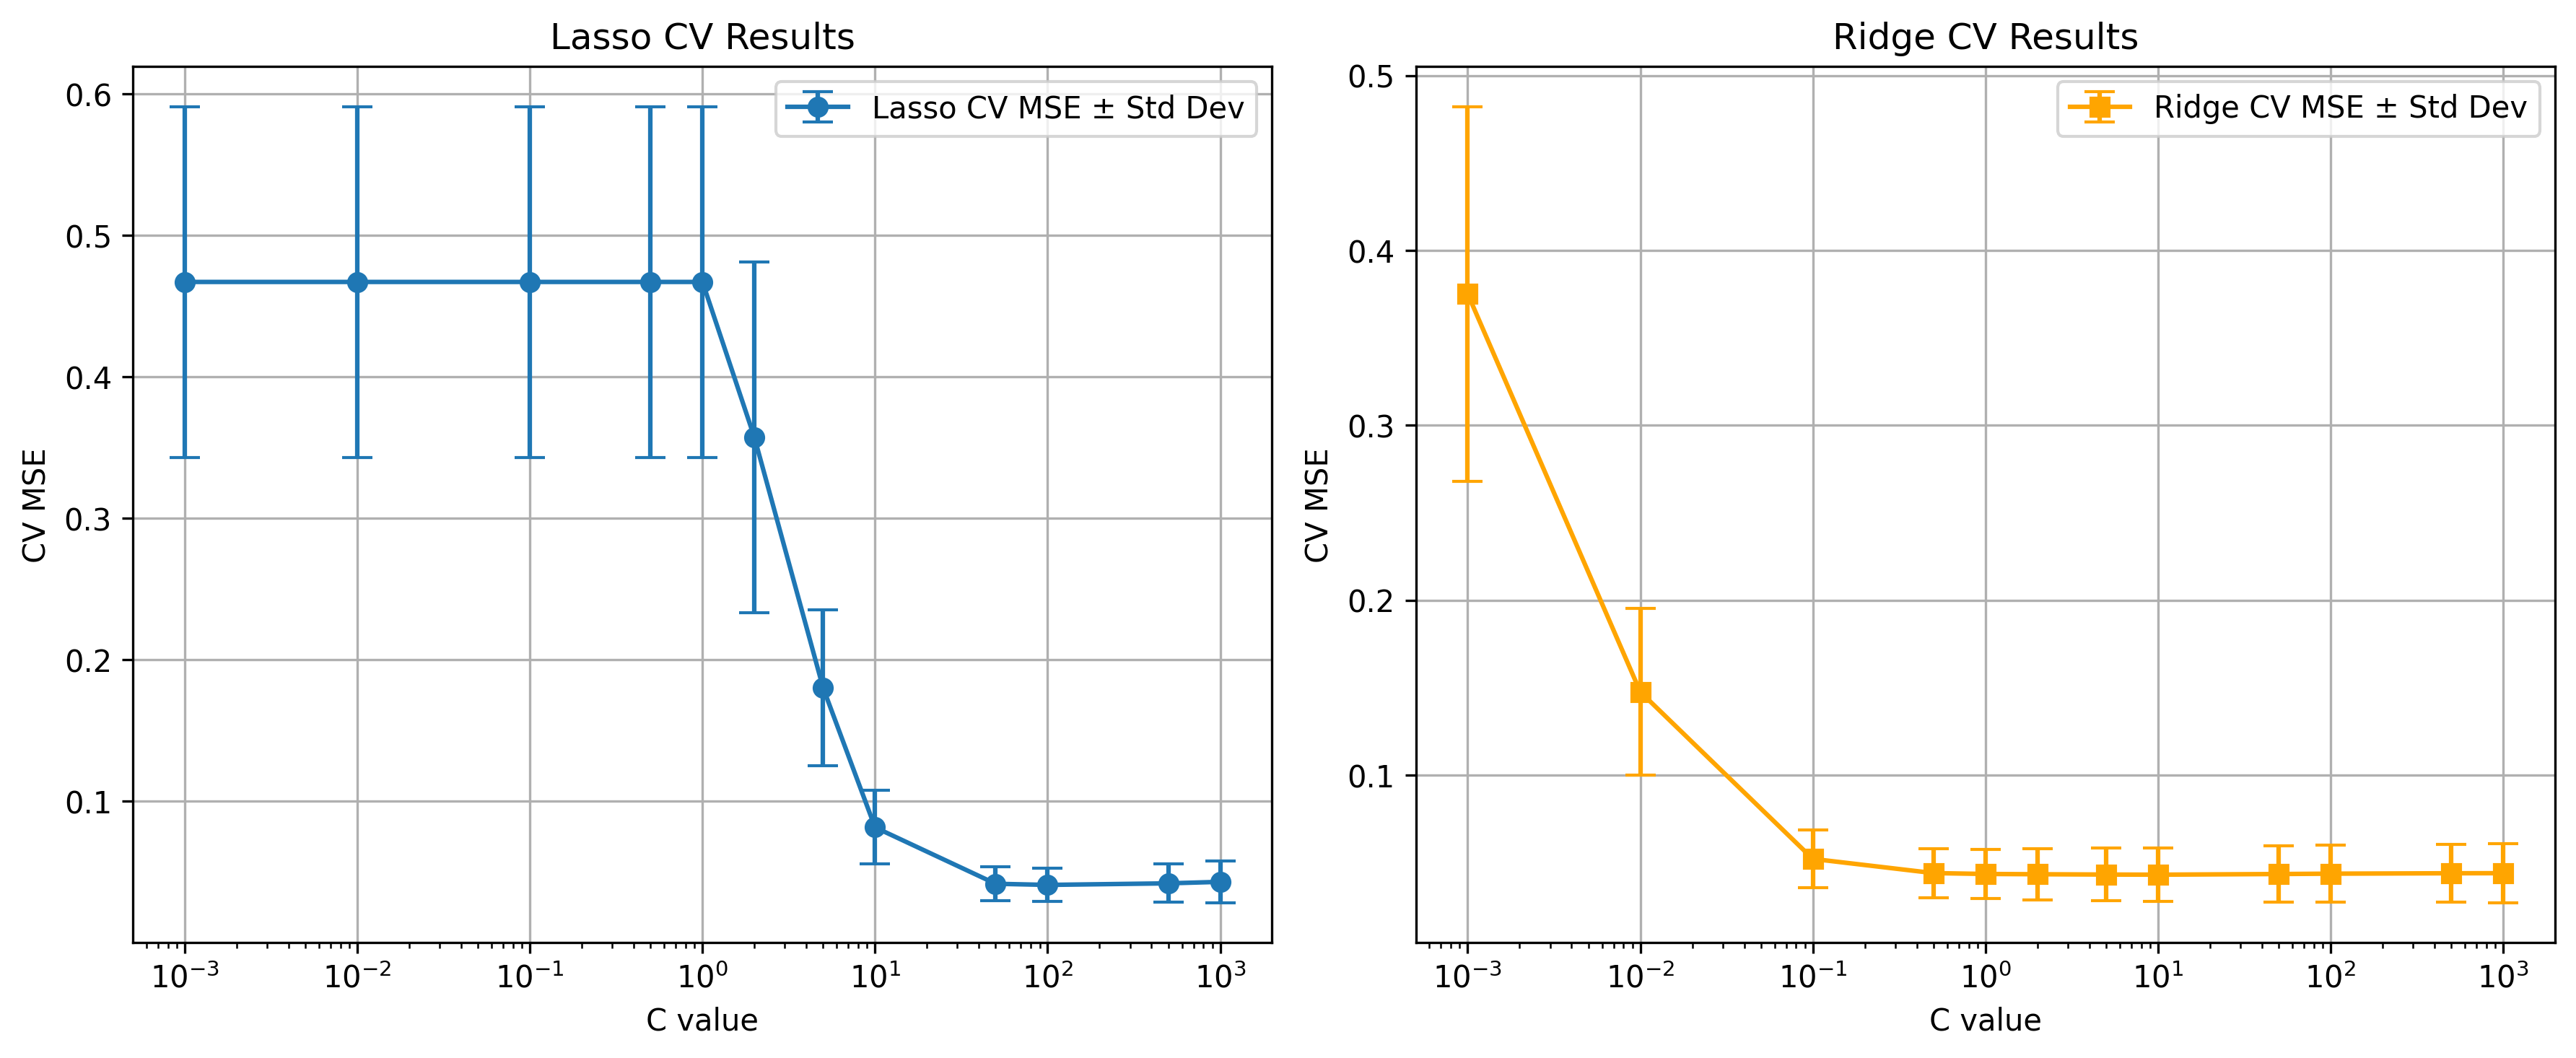
\includegraphics[width=0.95\textwidth]{figures/07_lasso_ridge_cv_comparison.png}
\caption{Side-by-side comparison of 5-fold CV results for Lasso (left) and Ridge (right). Lasso shows a sharp transition around C=2-10, while Ridge shows a smooth gradual improvement.}
\label{fig:cv_comparison}
\end{figure}

\section*{Final Comparison}

\textbf{Best Lasso Model:}
\begin{itemize}
    \item $C = 100$
    \item CV MSE = $0.0408 \pm 0.0119$
    \item Non-zero coefficients = 2/21
\end{itemize}

\textbf{Best Ridge Model:}
\begin{itemize}
    \item $C = 10$
    \item CV MSE = $0.0431 \pm 0.0154$
    \item Non-zero coefficients = 21/21 (all features used)
\end{itemize}

\textbf{Winner: Lasso performs slightly better} with about 0.0023 lower CV MSE.

But honestly both are pretty close. The choice between them depends on what you want:
\begin{itemize}
    \item If you want a \textbf{simpler, more interpretable model} $\rightarrow$ go with Lasso (only 2 features!)
    \item If you want \textbf{slightly more stable predictions} $\rightarrow$ Ridge might be better (smaller error bars at small $C$)
\end{itemize}

\begin{figure}[H]
\centering
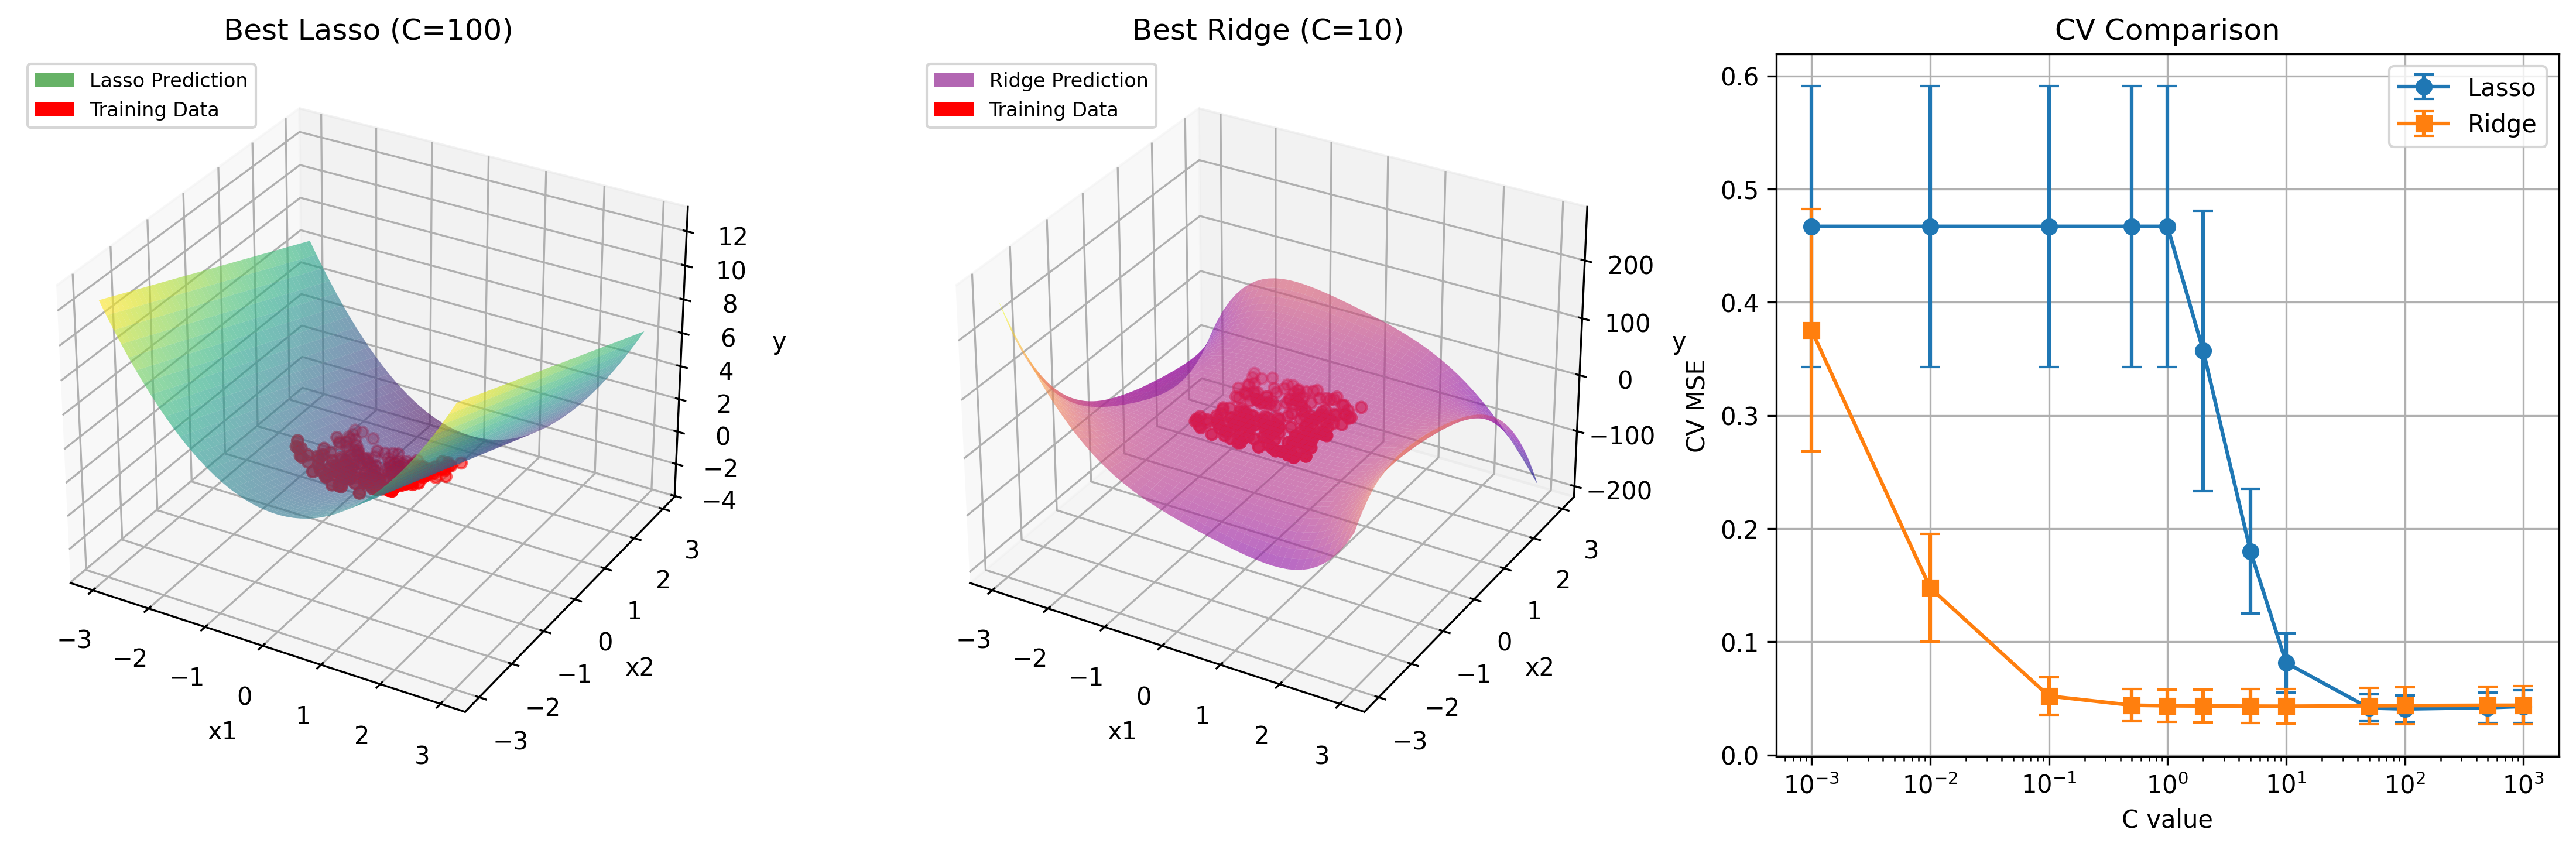
\includegraphics[width=\textwidth]{figures/08_final_comparison.png}
\caption{Final comparison: Left - Best Lasso model (C=100) with 2 features. Center - Best Ridge model (C=10) with all 21 features. Right - CV performance comparison showing both models achieve similar error rates.}
\label{fig:final_comparison}
\end{figure}

\section*{APPENDIX}

Code here will add later 

\end{document}

